% This is LLNCS.DOC the documentation file of
% the LaTeX2e class from Springer-Verlag
% for Lecture Notes in Computer Science, version 2.4
\documentclass{llncs}
\usepackage{llncsdoc}
\usepackage[hyphens]{url}
\usepackage[pdftex]{graphicx}     
\usepackage{float}
\usepackage{tablefootnote}
\usepackage{hyperref}



	%%%%%%%%%%%%%%%%%%%%%%%55
	%% Added to enable numbering for subsubsections, otherwise they would look like paragraphs which is ugly
	%%%%%%%%%%%%%%%%%%%%%%%55
	
	\makeatletter
	\renewcommand\subsubsection{\@startsection{subsubsection}{3}{\z@}%
		{-18\p@ \@plus -4\p@ \@minus -4\p@}%
		{0.5em \@plus 0.22em \@minus 0.1em}%
		{\normalfont\normalsize\bfseries\boldmath}}
	\makeatother
	\setcounter{secnumdepth}{3}

%
\begin{document}


	{
	%
	\title{We need a fancy title\\ \small Whitepaper - Version 0.1\\\small \today}
	
	\author{Benjamin Leiding\inst{1} \and Will Vorobev\inst{1} \and Peter Zverkov\inst{1} \and Lena Cherry\inst{1}}
	
	\institute{ 
		Chorus Technology
	}
	
	%\institute{University of G\"ottingen, Institute of Computer Science, G\"ottingen, Germany\\ benjamin.leiding@cs.uni-goettingen.de
	%\and
	%Tallinn University of Technology, Department of Informatics, Tallinn, Estonia\\
	%alex.norta.phd@ieee.org}
	
	\maketitle

	%% ----------------------------------------------------------------
	%% ----------------------------------------------------------------

	\begin{abstract}

		% A good abstract:
		%1.) What is the paper about?
		%2.) What is the SoA?
		%3.) What is the detected gap?
		%4.) What are the main questions to be answered pertaining to the gap?
		%5.) Why is the solution good/better than other solutions?

		
		I am an abstract - pet me.\\
		
		DON'T FORGET THE PLAGIARISM CHECK
		
	\end{abstract}
	
	
	\keywords{keywords}

	%% ----------------------------------------------------------------
	%% ----------------------------------------------------------------
	
	\section{Introduction}
		\label{s:introduction}

		Despite steadily growing public transport networks and systems, especially in most first world countries, cars and similar vehicles are still the default standard for urban transportation. In the US, ``about 86 percent of all workers commuted to work by private vehicle, either driving alone or carpooling" \cite{mckenzie2015drives} even though in recent years the numbers remained relatively stable after decades of consistent increase - similar applies to other industrial countries \cite{netherlandsPublicTransport}\cite{zealand2006car} even though the overall percentage of vehicle commuters in Europe is lower than in the US \cite{commuteUSvsEurope}. While it was normal for the last few decades to own a vehicle and commute on a day-by-day basis, the future will be radically different due to the progressing evolution of self-driving cars and autonomous vehicles. The car-sharing economy that developed in recent years in combination with autonomous cars results in a so called \textit{passenger economy} \cite{intelPassengerEconomy}. Users no longer own cars, instead just hop on an autonomous cars, pick a destination and get delivered without any human interaction. An Intel report estimates the size of this economy to be around US\$ 7 Trillion in 2050 \cite{intelPassengerEconomy}.
		
		Despite some recent setback, e.g. Uber and Tesla accidents \cite{bibid}\cite{bibid}\cite{bibid}, academic researchers as well as companies from the private sector make fast progresses in the research area of self-driving cars \cite{bibid}\cite{bibid}. It took less than 15 years from the first DARPA Grand Challenge (a prize competition for autonomous vehicles) to self-driving cars operating on public streets on a regular base (Tesla, Waymo, Uber, etc.) \cite{bibid}\cite{bibid}\cite{bibid}. Besides the cars, several projects are also already working on system solutions for trucks, rovers, drones, ships and even airplanes \cite{bibid}\cite{bibid}\cite{bibid}\cite{davWhitepaper}. But progressing automation and driverless transport that enables the passenger economy is only a small aspect of the potential of these new technologies. During a talk\footnote{\url{https://www.youtube.com/watch?v=MVyv4t0OKe4}} at the 2013 Turing Festival in Edinburgh, Mike Hearn did not only described a vision where most users don't own cars anymore and instead use services provided by autonomous vehicles that own itself, but also the potentials of a vehicle-to-vehicle (V2V) as well as a vehicle-to-infrastructure (V2I) economy. Autonomous vehicles (AVs) may own themselves, offer services and goods to earn money, and pay money to acquire services that they cannot provide on their own, e.g., car renting a parking lot, paying for a charged battery, using toll roads, or simple service check ups. The idea of V2V and V2I or in general V2X (vehicle-to-everything) will fuel various new business fields. 
		
		Certainly, traditional payment systems such as paper money or fiat currencies in general are not suited to be part of this new economy. There are slow, depend on third parties (e.g., banks) and suffer from bureaucratic overhead. Blockchain technology and cryptocurrencies offer a promising alternative payment solution that comes with several additional advantages that we will discuss later on. The blockchain technology, also referred to as distributed ledger system, is most noticeably known for providing the foundation of the peer-to-peer (P2P) cryptocurrency and payment system Bitcoin \cite{nakamoto_bitcoin:2008}, but nowadays there a various different platforms out there, e.g., \cite{tezosWhitepaper}\cite{iotaWhitepaper}\cite{wood2014ethereum}. Several companies already started to prototype applications that combine vehicles and blockchains. Porsche is researching different payment-related applications for vehicles \cite{porscheBlockchain} whereas Ford focuses on traffic marshaling \cite{macneille2018vehicle}. As expected in the early days of a new technology, companies focus on selective solutions for a selection of very specific problems or use cases and the resulting solutions are only compatible with their own products. What is currently missing in the new business field of V2X economy is an industry standard that can easily be integrated with self-driving and (semi)-autonomous cars or even nowadays cars. 

%https://www.heise.de/newsticker/meldung/Dubai-will-smarte-Kfz-Kennzeichen-testen-4016538.html

%%%%%%%%%%%%%%%%%%%%%%%%%%%%%%%%%%%%%%%%%%%%%%%%%%%%%%%%%%%%%%%%%%%%%%

%		RQ: How to implement a library for (semi)-autonomous vehicles that enables a V2X trading platform for goods and services?
%		RQ-1: What is the long term vision of Chorus Technology?
%		RQ-2: What are the critical requirements and the corresponding architecture of the Chorus platform?
%		RQ-3: What are the system-engagement processes for the stakeholders?


%%%%%%%%%%%%%%%%%%%%%%%%%%%%%%%%%%%%%%%%%%%%%%%%%%%%%%%%%%%%%%%%%%%%%%

		This whitepaper addresses the detected gap by introducing the Chorus Technology solution, thereby answering the question of how to implement a library for (semi)-autonomous vehicles that enables a V2X trading platform for goods and services? In order to answer this question with a separation of concerns, we pose the following sub-questions: What is the long term vision of Chorus Technology? What are the critical requirements and the corresponding architecture of the Chorus platform? What are the system-engagement processes for the stakeholders?

		The remainder of this paper is structured as follows: Section~\ref{s:section-2} introduces supplementary literature and related work. Section~\ref{s:section-3} then outlines the vision of Chorus Technology as well as different use-cases. Afterwards, Section~\ref{s:section-4} analyses the requirements of the our system and outlines the resulting system architecture that we derive from the requirements. Afterwards, Section~\ref{s:section-5} expands on the system-engagement processes for the stakeholders, followed by Section~\ref{s:section-6} that introduces the Chorus prototype as well as feasibility evaluation. Section~\ref{s:section-7} provides an discussion and an analysis of related projects. Finally, Section~\ref{s:section-8} concludes this work and provides an outlook on future work.


	%% ----------------------------------------------------------------
	%% ----------------------------------------------------------------

	\section{Technical Background and Supplementary Literature}	
		\label{s:section-2}
		
		The following section provides background information and describes related works regarding previous ideas and concepts that focus on a blockchain-based VANET platforms. First, Section~\ref{ss:blockchain-intro} introduces the general concepts of blockchain technology, terms and frameworks. Afterwards, Section~\ref{ss:autonomous-vehicles} and Section~\ref{ss:vanets} focus on the fundamentals of autonomous vehicles as well as vehicular ad-hoc networks.
					
		%% ----------------------------------------------------------------
		%% ----------------------------------------------------------------	
		
		\subsection{Blockchain Technology}
			\label{ss:blockchain-intro}
			
			As the name suggests, a blockchain consists of a chronologically ordered chain of blocks. Every block consists of a certain number of validated transactions and each of those block links to its predecessor by a hash reference. As a result, changing the content of one block also changes all succeeding blocks and hence breaks the chain. All blocks are stored on and verified by all participating nodes. While the initial Bitcoin blockchain only supported a very limited set of scripting instructions, the next generation of blockchain platforms, e.g., Ethereum \cite{wood2014ethereum}, Qtum \cite{qtumWhitepaper}, or Tezos \cite{tezosWhitepaper}, provide Turing-complete programming languages on the protocol-layer level in order to enable smart contract capabilities. Smart contracts are, ``orchestration- and choreography protocols that facilitate, verify and enact with computing means a negotiated agreement between consenting parties" \cite{qtumWhitepaper}. Hence, the parties participating in the enactment of a smart contract establish binding agreements and deploy applications using such smart contracts in order to provide blockchain-based applications. Those application are as versatile as smart contracts itself and enable services including the finance sector \cite{nguyen2016blockchain}\cite{saltWhitepaper}, academic and business authentication and identity solutions \cite{leidingUnchained}\cite{CivicWhitepaper}\cite{AuthcoinLeiding2016MCIS}\cite{mccorry2015authenticated}\cite{SelfkeyWhitepaper}, reputation systems \cite{SemadaWhitepaper} as well platforms for Internet-of-Things (IoT) applications \cite{christidis2016blockchains}\cite{ouaddah2017towards}. 	
			
			The blockchain concept is particularly interesting for the V2X economy for three reasons. First, it removes the need for trusted third parties and instead enables trust-less transaction enactment. Second, transactions that were agreed up on cannot be changed any more since the underlying blockchain is tamperproof. Third, no human interaction is required for any kind of transaction between vehicles or machines in general.

		%% ----------------------------------------------------------------
		%% ----------------------------------------------------------------	
		
		\subsection{Autonomous Vehicles}
			\label{ss:autonomous-vehicles}
			
			During the last 15 years research on autonomous and self-driving cars progressed a lot and nowadays such cars already operating on public streets on a regular base, e.g., Tesla, Waymo, Uber, and so on. The ultimate goal of most manufacturers and researchers is to develop the first fully self-driving and autonomous vehicle. In order to clarify some definitions, this short section provides a short introduction to the most relevant terms and concepts.

			An autonomous car, also referred to as a driverless car or robotic car, is able to navigating and interact with its environment without human input based on information provided by its sensors \cite{gehrig1999dead}\cite{thrun2010toward}. To do so, modern cars are equipped with radar- and laser sensors, lidars, GPS devices, cameras and several further sensing devices. Based on these information, the vehicle interprets the surrounding world and deduces appropriate action strategies such as avoiding obstacles (other vehicles, humans or a house) on the way to the supermarket \cite{dokic2015european}\cite{zhu2014vehicle}. As the technology developed over time, vehicles were equipped with more and more sensors, resulting in different driving capabilities. The SAE \cite{autonomyLevelsSAE}
			defined six levels of driving autonomy to categorize the varying capabilities and progresses of several approaches:		
			
			\begin{itemize}
				\item \textbf{Level 0 (No automation): }No driving autonomy, the driver has to perform all driving tasks and interactions.
				\item \textbf{Level 1 (Driver assistance): }The vehicle is controlled by the driver, but is supported by some basic driver assistance functionalities.
				\item \textbf{Level 2 (Partial automation): }The vehicle is able to perform some specific tasks (acceleration or steering) without driver input. Nevertheless, the driver must be fully engaged in driving task and monitor all decision of the car and the environment at all time. The user has to be able to intervene at any given moment. 
				\item \textbf{Level 3 (Conditional automation): }The driver is still a necessity, but is not required to monitor the vehicle or the environment at any given moment. But given a notification by the vehicle, the driver has to be able to take back control over the car in case the vehicle encounters a situation that it cannot deal with on its own.
				\item \textbf{Level 4 (High Automation): }The vehicle is able to perform all driving tasks without human intervention in most driving scenarios. The driver can take control whenever desired.
				\item \textbf{Level 5 (Full Automation): }The vehicle is able to perform all driving tasks without human intervention in all driving scenarios. The driver can take control whenever desired as long as a steering wheel is still part of the vehicle.
			\end{itemize}
			
			The Chorus interaction- and transaction layer library supports and enables a varying number of services for vehicles of each automation level, whereas the most sophisticated applications require SAE level 5 and simpler plug-ins may only require SAE level 1.

		%% ----------------------------------------------------------------
		%% ----------------------------------------------------------------	
		
		\subsection{Vehicular Ad-Hoc Networks - VANETs}
			\label{ss:vanets}

			Communication between vehicles, road infrastructure and Internet-based services is a key enabler of upcoming generation of vehicles. So called vehicular ad-hoc networks provide an abstract concept that models the different components that are required for V2V, V2I and V2X communication. As illustrated in Figure \ref{fig:vanets}, the basic components of VANETs are vehicles, on-board-units (OBUs), application-units (AUs) and road-side-units (RSUs).\\
			RSUs are placed  along the road side or in dedicated locations such as at crossroads. Usually, RSUs provide short range communication based on IEEE 802.11p radio technology but can also be equipped with other network devices in order to provide communication within the infrastructural network \cite{al2014comprehensive}. An OBU is typically mounted onto a vehicle and used for exchanging information with RSUs or other OBUs. Short range wireless communication or other radio technologies are usually used to exchange information \cite{baldessari2007car}.\\
			Closely linked to the OBU is the AU. They might even reside in the same physical unit or is mobile and might be regularly removed from the vehicle (e.g smartphones). The AU provides an execution environment for applications that utilize the OBU's communication capabilities \cite{al2014comprehensive}\cite{baldessari2007car}.\\	
			\begin{figure}[ht]
				\centering
				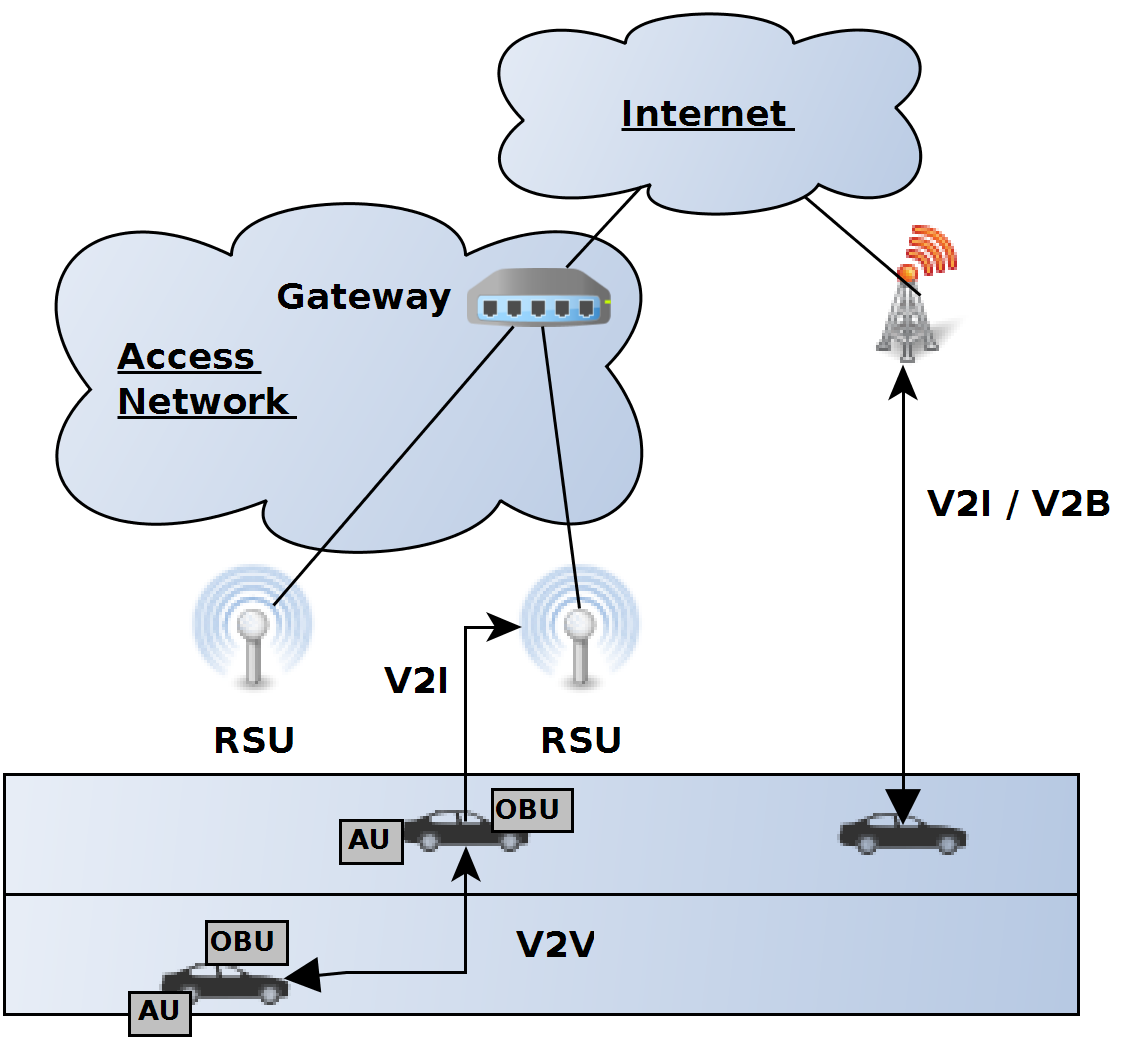
\includegraphics[scale=0.2]{Figures/Vanets.png}
				\caption{General VANET architecture (Based on: \protect\cite{baldessari2007car} and \cite{leiding2016self})}
				\label{fig:vanets}
			\end{figure}			
			Communication in VANETs occurs either inside a vehicle between AUs and OBU, wirelessly between different vehicles (V2V), vehicles and infrastructure (V2I) or vehicles and the infrastructure via broadband (V2B) \cite{faezipour2012progress}. For authentication purposes, each network participant is equipped with a unique public/private key pair which usually resides in a tamper-proof-device (TPD). In blockchain terms, the TPD is similar to an external hardware wallet.
			
		%% ----------------------------------------------------------------
		%% ----------------------------------------------------------------	
		
%		\subsection{Related Work}
%			\label{ss:related-work}
%
%			\textbf{Work-In-Progress}
%
%			
%
%
%		%% ----------------------------------------------------------------
%		%% ----------------------------------------------------------------	
%	

	%% ----------------------------------------------------------------
	%% ----------------------------------------------------------------

	\section{The Chorus Vision}
		\label{s:section-3}
		
		%%RQ-1: What is the long term vision of Chorus Technology?
		
		Intro

		%foam and localization somewheere here	

		%% ----------------------------------------------------------------
		%% ----------------------------------------------------------------	
		
		\subsection{Use Cases}
			\label{ss:use-cases}

			\textbf{Work-In-Progress}
			
			CHECK THE chorus website for this section
			
		\subsection{Human to Human}

		\subsection{Human to Vehicle}
		
		\subsection{Vehicle to Vehicle}
			\label{ss:V2V}
			
				road space negotiation
			
		\subsection{Vehicle to Infrastructure}					
		
		%% ----------------------------------------------------------------
		%% ----------------------------------------------------------------	


	%% ----------------------------------------------------------------
	%% ----------------------------------------------------------------
	
	
	\section{System Design and Architecture}
		\label{s:section-4}	

		%%RQ-2: What are the critical requirements and the corresponding architecture of the Chorus platform?

		The vision of Chorus outlined in Section \ref{s:section-3} is now analyzed from technical perspective as part of the following section. In order to identify, structure and formalize the critical requirements and stakeholders on an abstract level, we use one part of an Agent-Oriented Modeling (AOM) method \cite{sterling2009art}, i.e., goal models. Section~\ref{ss:requirement-engineering} introduces AOM goal models and the Chorus specific goal model. The produced goal model is used in subsequent Section \ref{ss:component-diagrams} to derive the Chrous system architecture . The resulting system architecture and specifications serve as implementation guidelines. Finally, Section~\ref{ss:smart-contract-lifecycle-management} provides some details on the smart contract lifecycle management within our solution, whereas Section~\ref{ss:library-api} outlines a general outlook on the APIs and how to integrate the Chorus library into external applications.
		
		
		%% ----------------------------------------------------------------
		%% ----------------------------------------------------------------	
		
		\subsection{Functional Goals, Quality Goals, Stakeholders and Requirements}
			\label{ss:requirement-engineering}
						
			In system development and software engieerng, good requirements follow certain characteristics. According to \cite{davis1993software}\cite{ieee1994ieee} requirements address one issue only and are completely specified without missing information. Moreover, they have to be consistent and do not contradict itself, or in correlation with other requirements. Finally, a requirement must also be atomic and without conjunctions \cite{norta2014reference}.

			\begin{figure}[H]
				\centering
				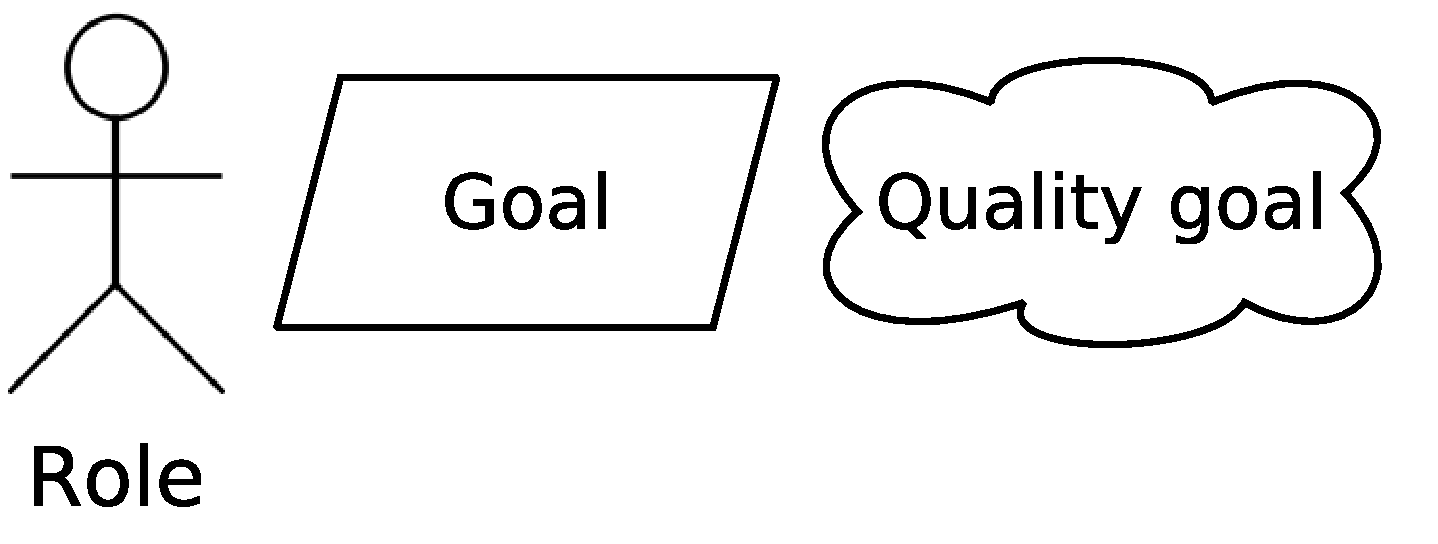
\includegraphics[scale=0.2]{Figures/20180426_AOM-notation.pdf}
				\caption{Selection of AOM notation elements.}	
				\label{fig:aom-notaion-elements}
			\end{figure}				
			The AOM methodology is a socio-technical requirements-engineering approach used to model complex systems that consist of humans, devices, and software agents. An AOM goal model enables both, technical- and non-technical stakeholders, to capture and understand the functional- and non-functional requirements of a complex system. Figure \ref{fig:aom-notaion-elements} depicts the three main elements that an AOM goal model comprises in order to capture the system requirements and goals. Roles of involved entities are represented in form of sticky men, whereas functional requirements are depicted as parallelograms. Note that in the specific context of this whitepaper, a sticky man does not exclusively represent human entities but rather all kinds of entities, e.g., also vehicles or infrastructure. Functional requirements are also referred to as goals. Non-functional requirements are depicted as clouds and refer to quality goals of the modeled software system. The AOM goal model follows a tree-like hierarchy with the root value proposition of the modeled system at the top. Subsequently, this main goal is decomposed into sub-goals where each sub-goal represents an aspect for achieving its parent goal \cite{marshall2014agent}. The goals are further decomposed into multi-layered sub-goals until the lowest atomic level is reached. Additionally, roles and quality goal may be assigned to goals and are inherited to lower-level goals. The following Section~\ref{sss:top-level-goal-model} introduces the top-level goal model our system, followed by Section~\ref{sss:quality-goals} focusing on the non-functional goals of the AOM goal model.

			
			%% ----------------------------------------------------------------
			%% ----------------------------------------------------------------	
					
			\subsubsection{Top-Level AOM Goal Model}
				\label{sss:top-level-goal-model}
				
				The presented AOM goal model is similar to the model presented by the authors in \cite{leidingM2M}, since implementation of a V2X system is a specific use case of the more abstract and general M2M (machine-to-machine) interaction platform represented in that paper. Meanwhile, Figure \ref{fig:top-level-aom-goal-model} presents the top-level AOM goal model of the system using the modeling method described above. The main value proposition is to provide a V2X interaction and transaction layer library for (autonomous) vehicles, thereby representing the root of the goal model. The complex main value proposition is split into four sub-goals representing the four main components.
				
				First, one component for managing the V2X platform. This functional goal includes managing certain aspects of the platform itself, e.g., creating, updating, deleting a new platform, as well as the management of the underlying smart contracts. Each platform operates a master smart contract and several sub-smart contracts. While the master contract is in charge of platform management and controlled by the hardware vendor (e.g., Tesla), the sub contracts each offer service provision for a specific service, interaction, transaction or application.
				
				The second functional goal enables V2X interaction. That mostly covers on- and off-chain supply and demand administration. Entities may register offers or requests on-chain in order to attract business partners, but for the other use cases a local supply demand management off-chain is more suitable, e.g., road-space negotiation. Supervising on- and off-chain auctions is basically equivalent to the on- and off-chain supply and demand management. Besides that, plug-ins and dApps of the Chorus eco-system might use platform smart contracts for service enactment and have to be integrated as well in this context.
				
				The third functional requirement, that represents the third main component, enables V2X transaction via the blockchain. The most important part here is the transaction management via a smart contract lifecycle that will be detailed later on in Section \ref{ss:smart-contract-lifecycle-management}.
				
				Finally, the fourth functional requirement focus on the enactment of various plug-ins and decentralized applications (dApps). Applications and plug-ins have to be registered, prepared for enactment, executed and terminated. Moreover, they have to interact with various entities of the eco-system depending on the use case. Since nowadays most blockchains offer Turing-complete smart contract support, the variety of applications and plug-ins in our eco-system is quite vast. 
				
%				\begin{figure}[H]
%					\centering
%					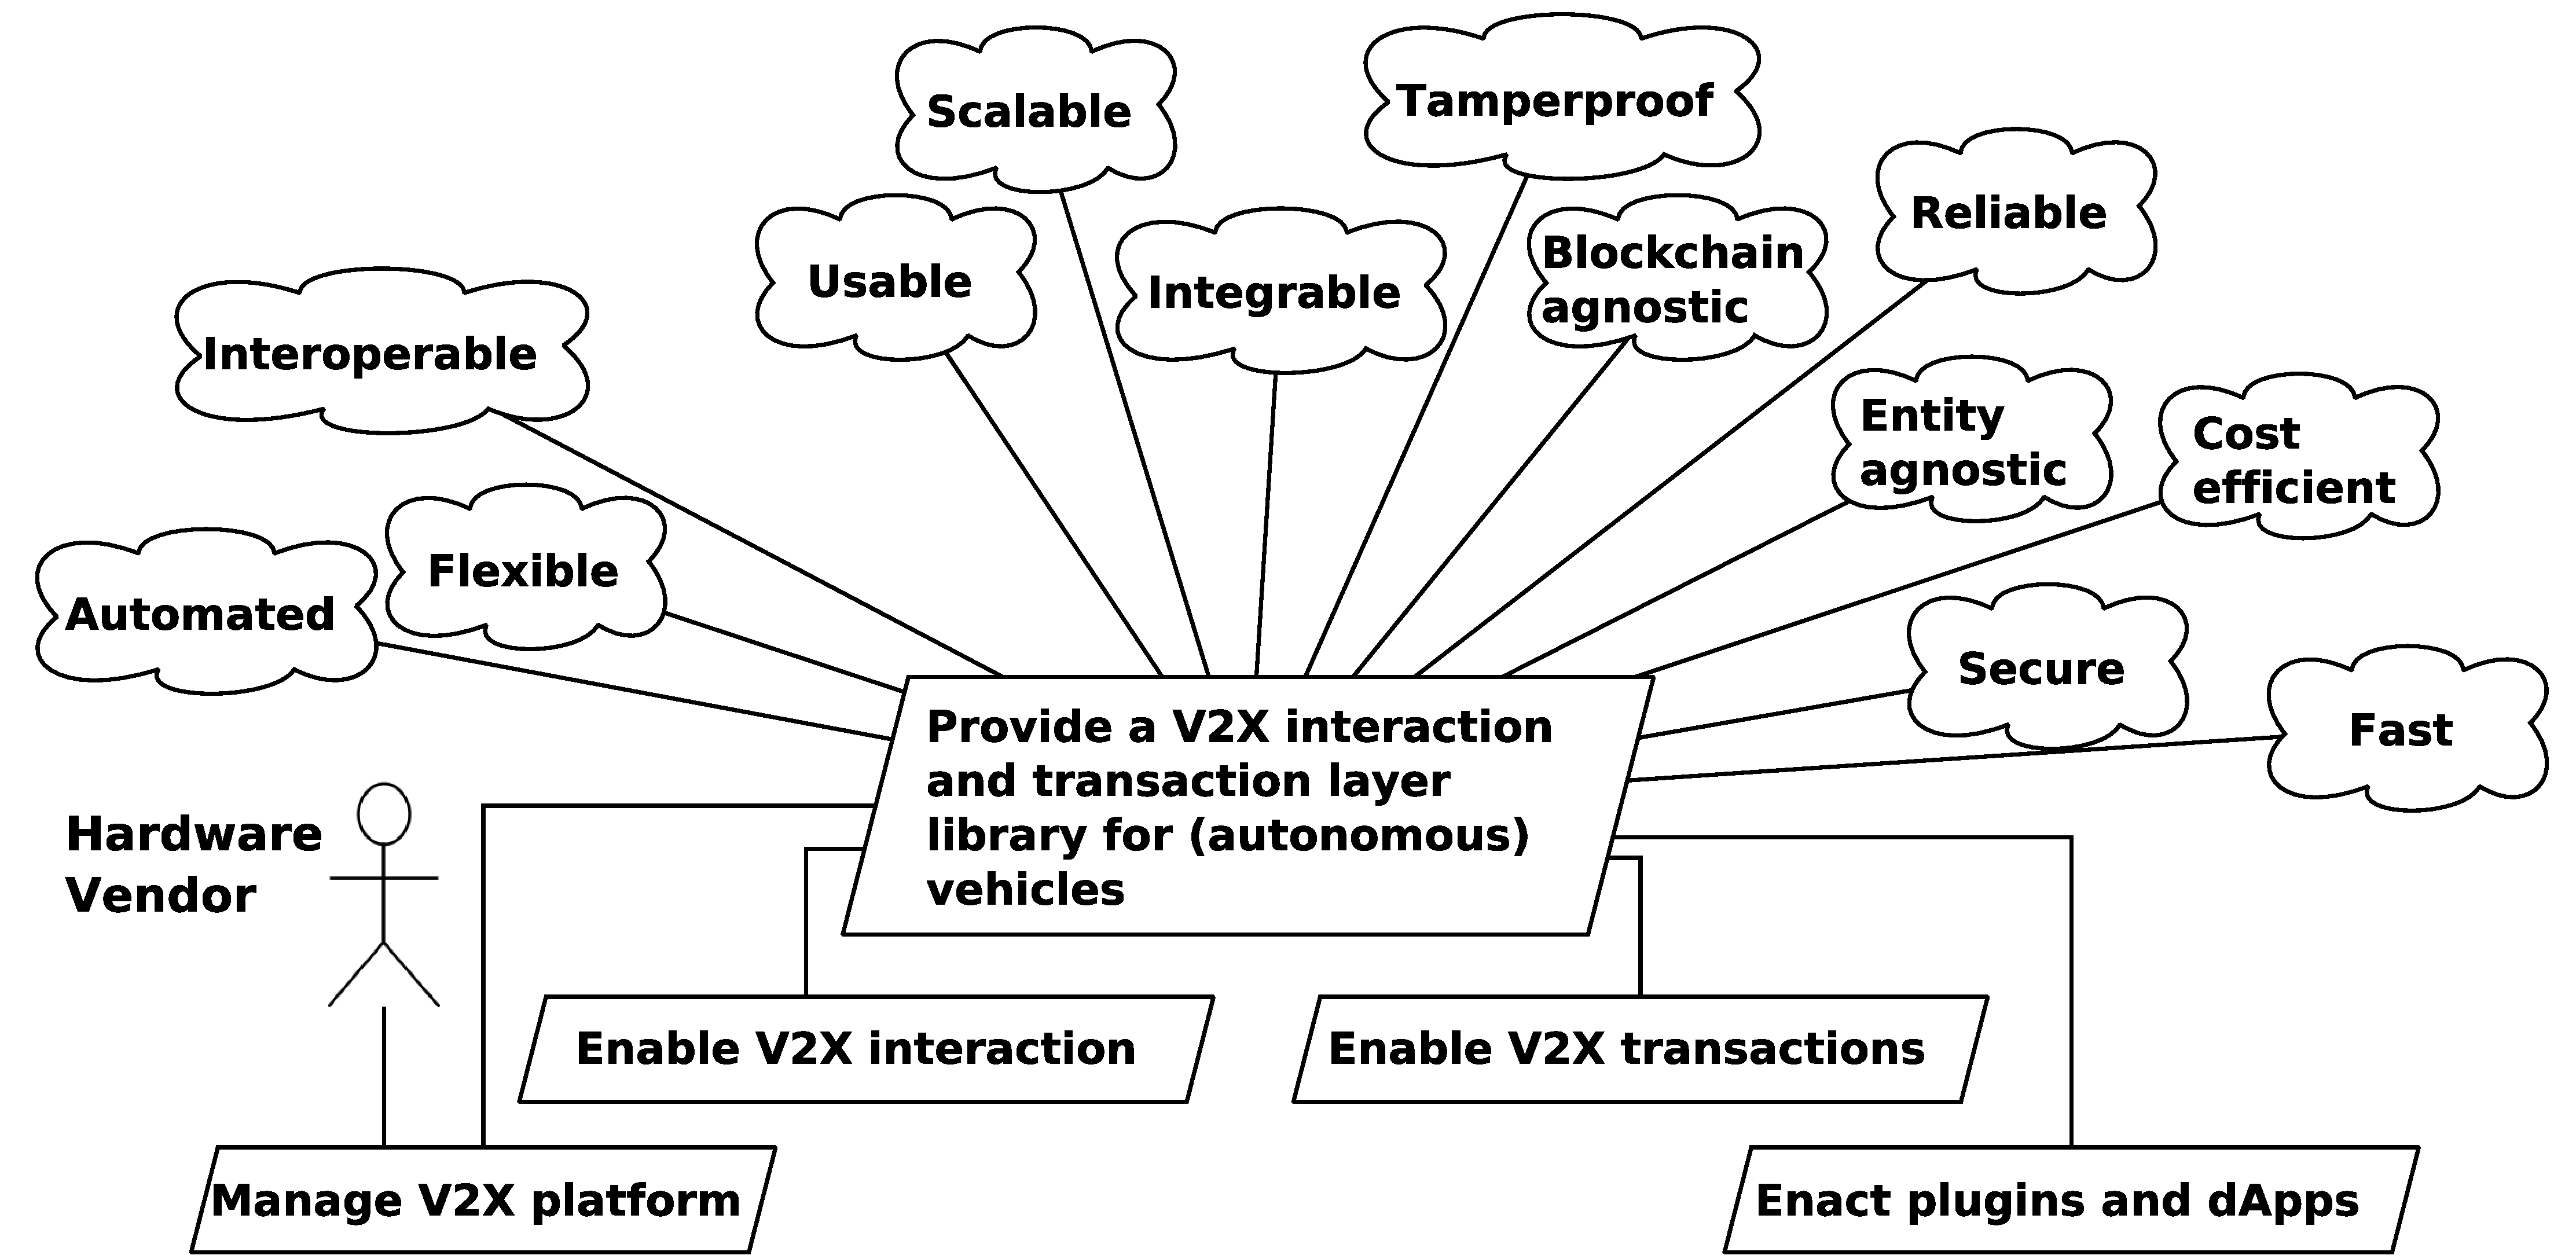
\includegraphics[scale=0.15]{Figures/aom/20180501_goal-model--top-level.pdf}
%					\caption{Chorus - Top-level goal model representation (Source: Based on \cite{leidingM2M}).}	
%					\label{fig:top-level-aom-goal-model}
%				\end{figure}
				
				\begin{figure}[H]
					\centering
					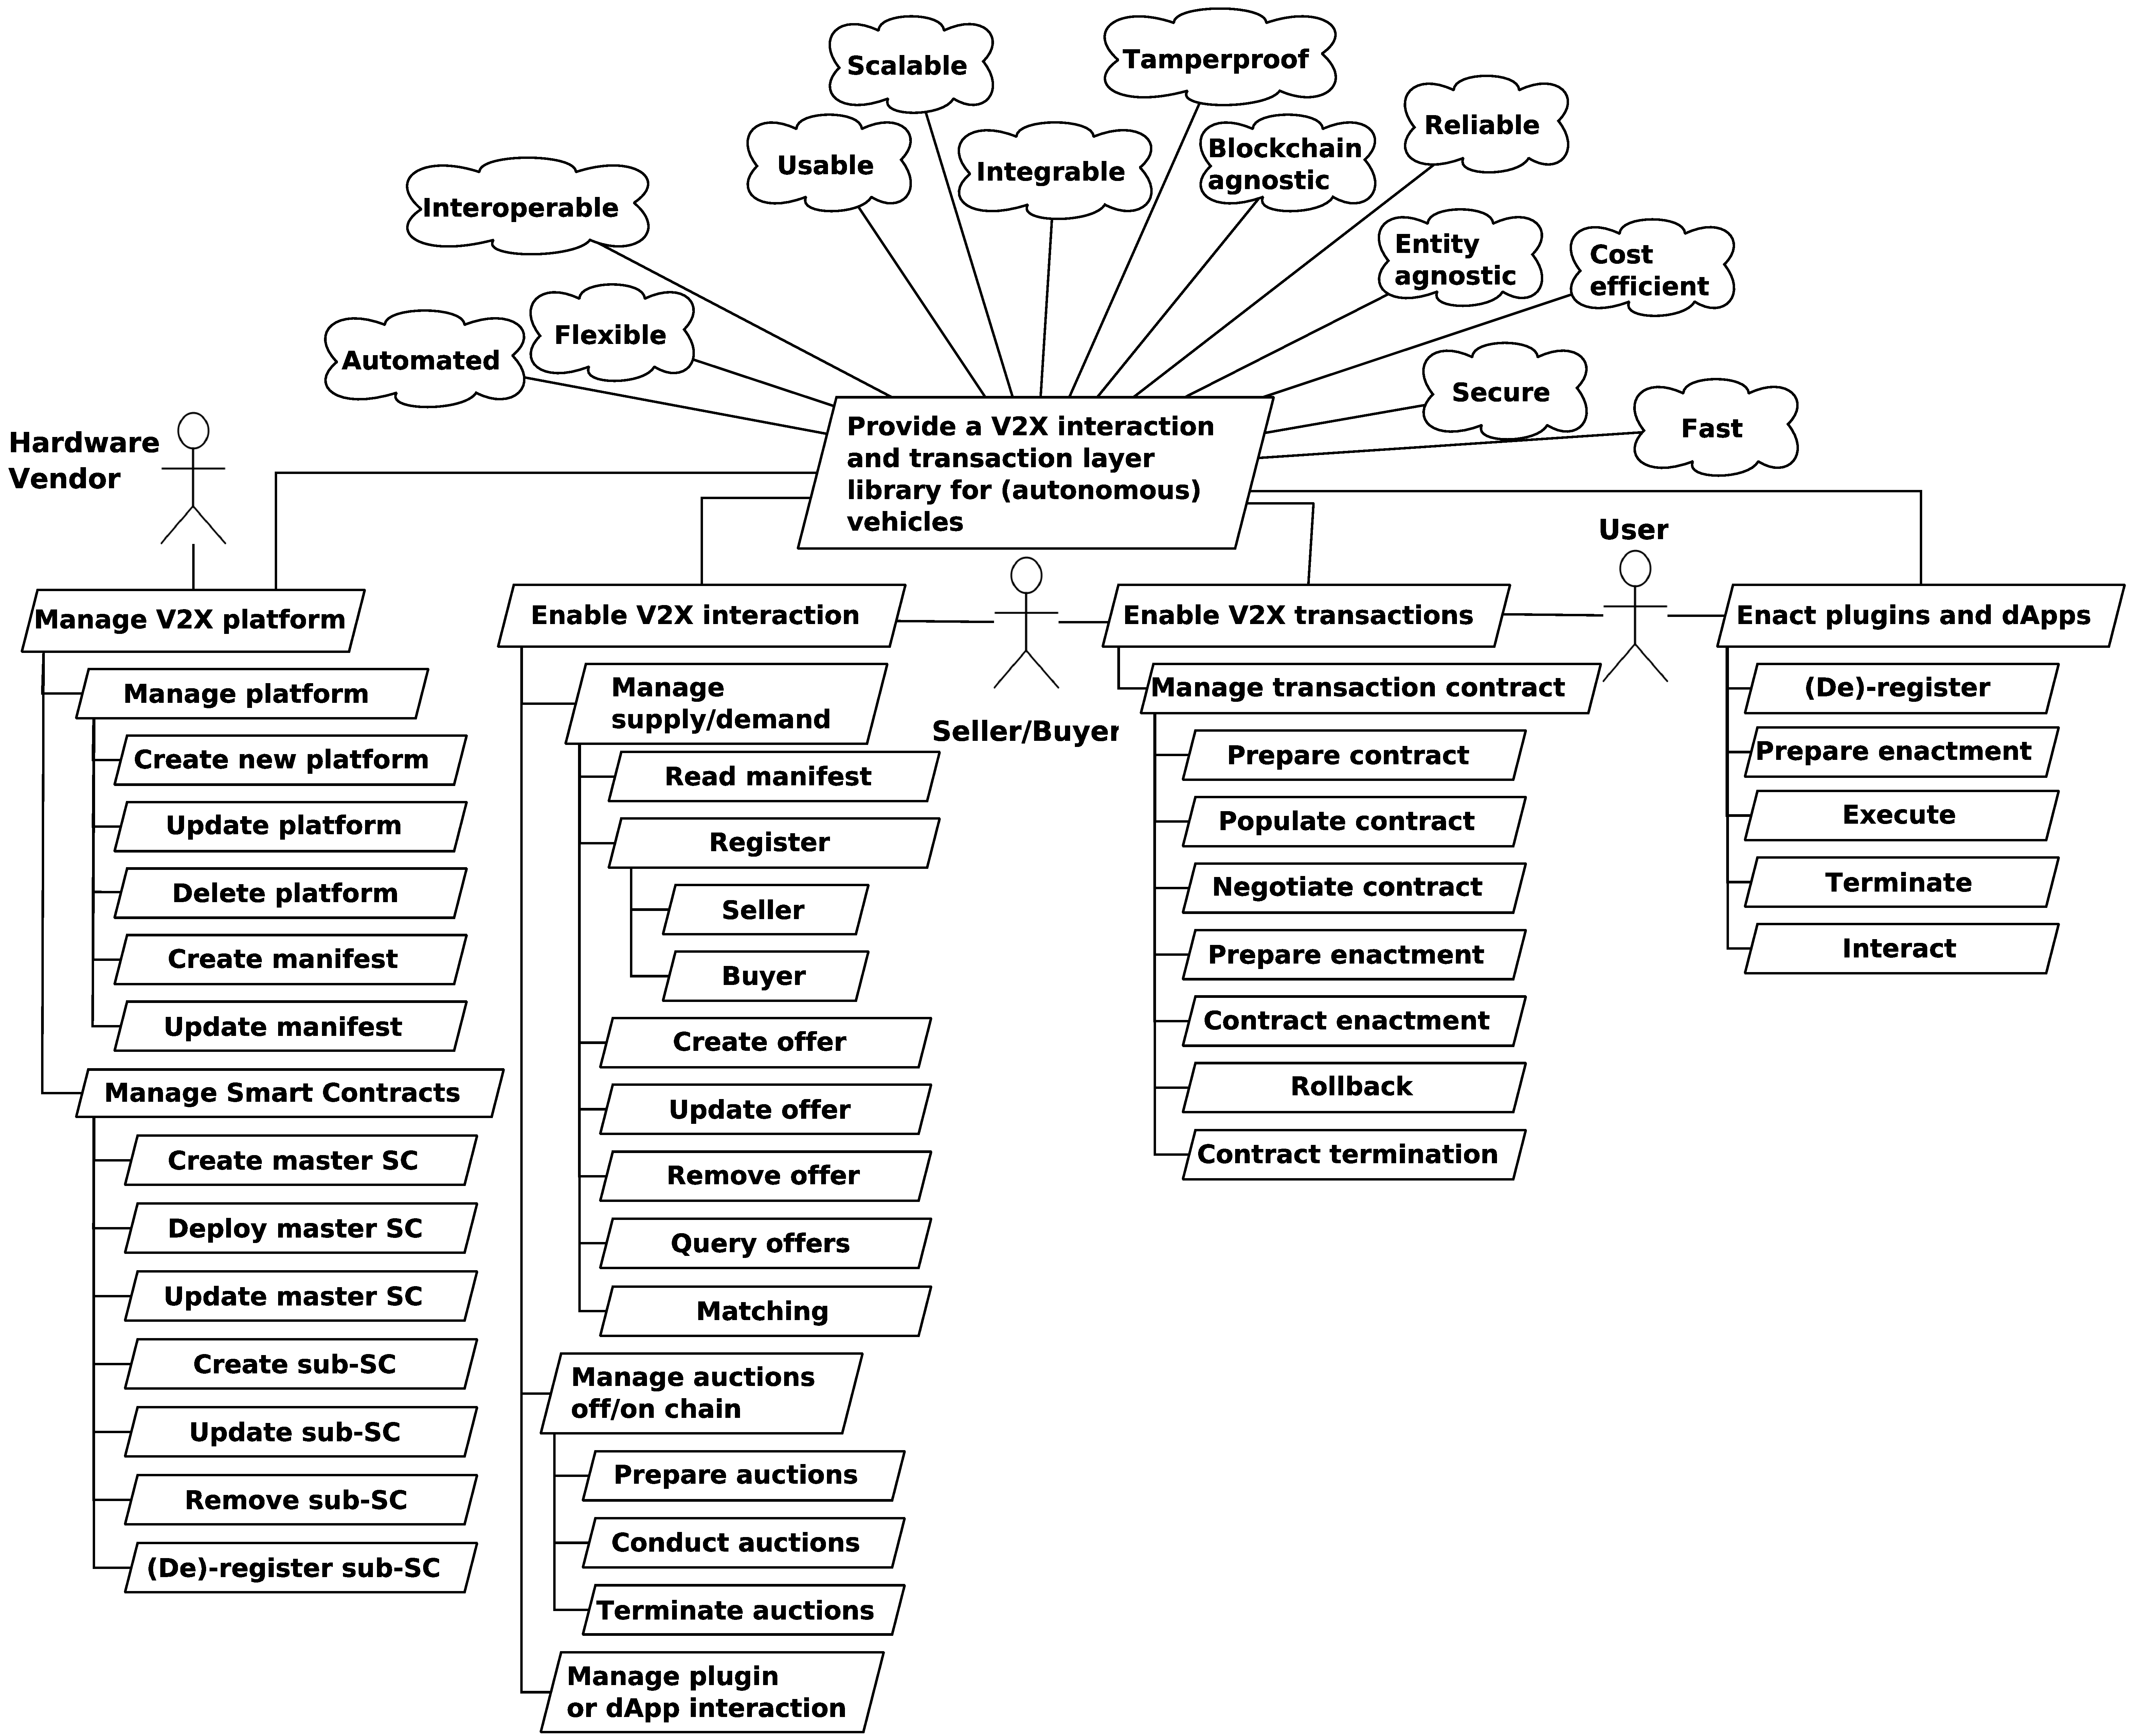
\includegraphics[scale=0.13]{Figures/aom/20180501_goal-model--complete.pdf}
					\caption{Chorus - Top-level goal model representation (Source: Based on \cite{leidingM2M}).}	
					\label{fig:top-level-aom-goal-model-extended}
				\end{figure}				

			\subsubsection{Non-Functional Requirements}
				\label{sss:quality-goals}
								
				Besides the four sub-goals of the top-level AOM goal model, we further identify thirteen quality goals of the main value proposition that are inherited to all refining sub-goals. A \textit{scalable} system design is necessary to provide Chorus services to a large quantity of users and customers. A further property that supports to achieve this scalability is the non-functional requirement \textit{automated}, that refers to a high degree of process automation eliminating the need for human interaction, e.g., tedious and repetitive tasks. \textit{Cost efficiency} is another important quality goal. \textit{Flexible} digital collaboration is a highly dynamic process that involves the enactment of diverse activities, the participation of diverse partners, and the exchange of diverse data \cite{norta2008exploring}. Thus, we must allow diverse collaboration scenarios and permit the inter-organizational harmonization of heterogeneous concepts and technologies between participating entities. Another key property of the system being easy to use (\textit{Usable}) for business collaboration. According to \cite{norta2014reference}, easy usability also includes the support of proper \textit{error avoidance} in order to ``anticipate and prevent common errors that occur during a collaboration configuration. Closely related is \textit{error handling}, to help with system support a user to recover from errors. \textit{Learnability} refers to how quickly users master using the system" \cite{norta2014reference}. 
				
				Moreover, we assign two additional quality goals that ensure a \textit{blockchain agnostic} as well as \textit{entity agnostic} design. Chorus should be neither limited to a specific blockchain nor vehicle hardware of a specific vendor. \textit{Interoperable} hardware and software design is another consequence of the previous quality goals as well as easy integration (\textit{Integrable}). It is crucial to interoperate at runtime with information systems supporting other business functions.
				
				Furthermore, a \textit{secure} service provision is also crucial in terms of operational security, e.g., protect user accounts and personal data from unauthorized access, secure data transfer within the system between entities or preventing data- and information leaks as well as preventing accidents. A \textit{reliable} enactment of all Chorus-based interactions and transaction facilitates the previous goals as well. Data communicated internally as well as externally has to protected against unauthorized tampering (\textit{tamperproof}) in order to protect business collaborations, but also ensure the safety of participating entities. Finally, since cars and similar vehicles move much faster than humans, a \textit{fast} service provision is essential for most tasks.
			
			%% ----------------------------------------------------------------
			%% ----------------------------------------------------------------	
					
%			\subsubsection{Refined AOM Goal Model}				
%				\label{sss:refined-goal-model}			
%
%				\begin{figure}[H]
%					\centering
%					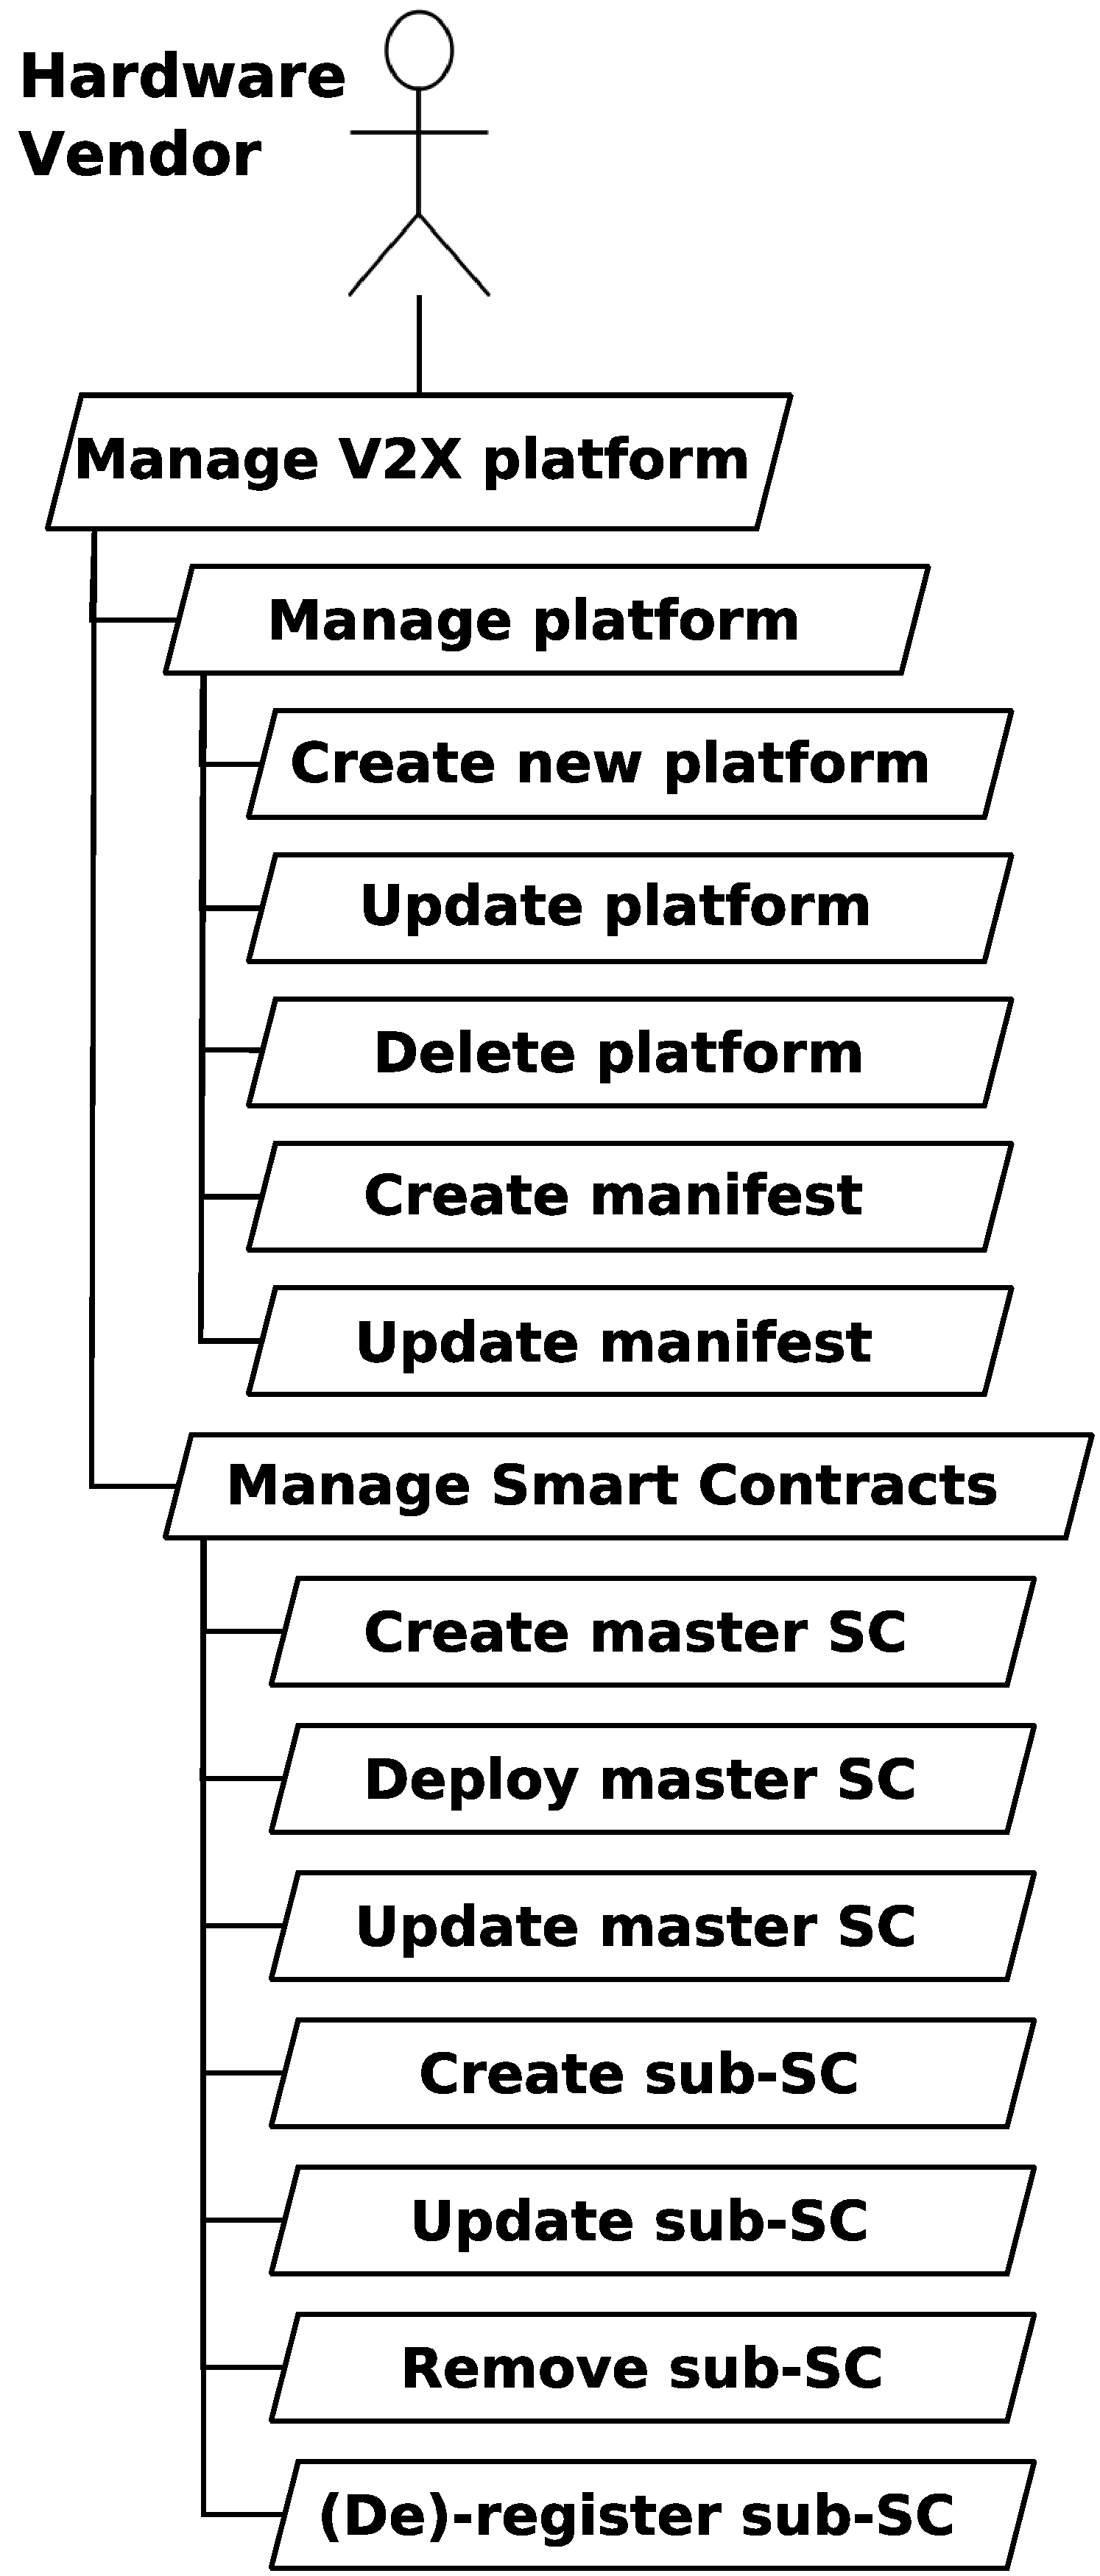
\includegraphics[scale=0.175]{Figures/aom/20180501_goal-model--refined-1.pdf}
%					\caption{Chorus - Goal model refinement \textit{Manage V2X platform} (Source: Based on \cite{leidingM2M}).}	
%					\label{fig:refined-aom-goal-model-1}
%				\end{figure}
%				
%				\begin{figure}[H]
%					\centering
%					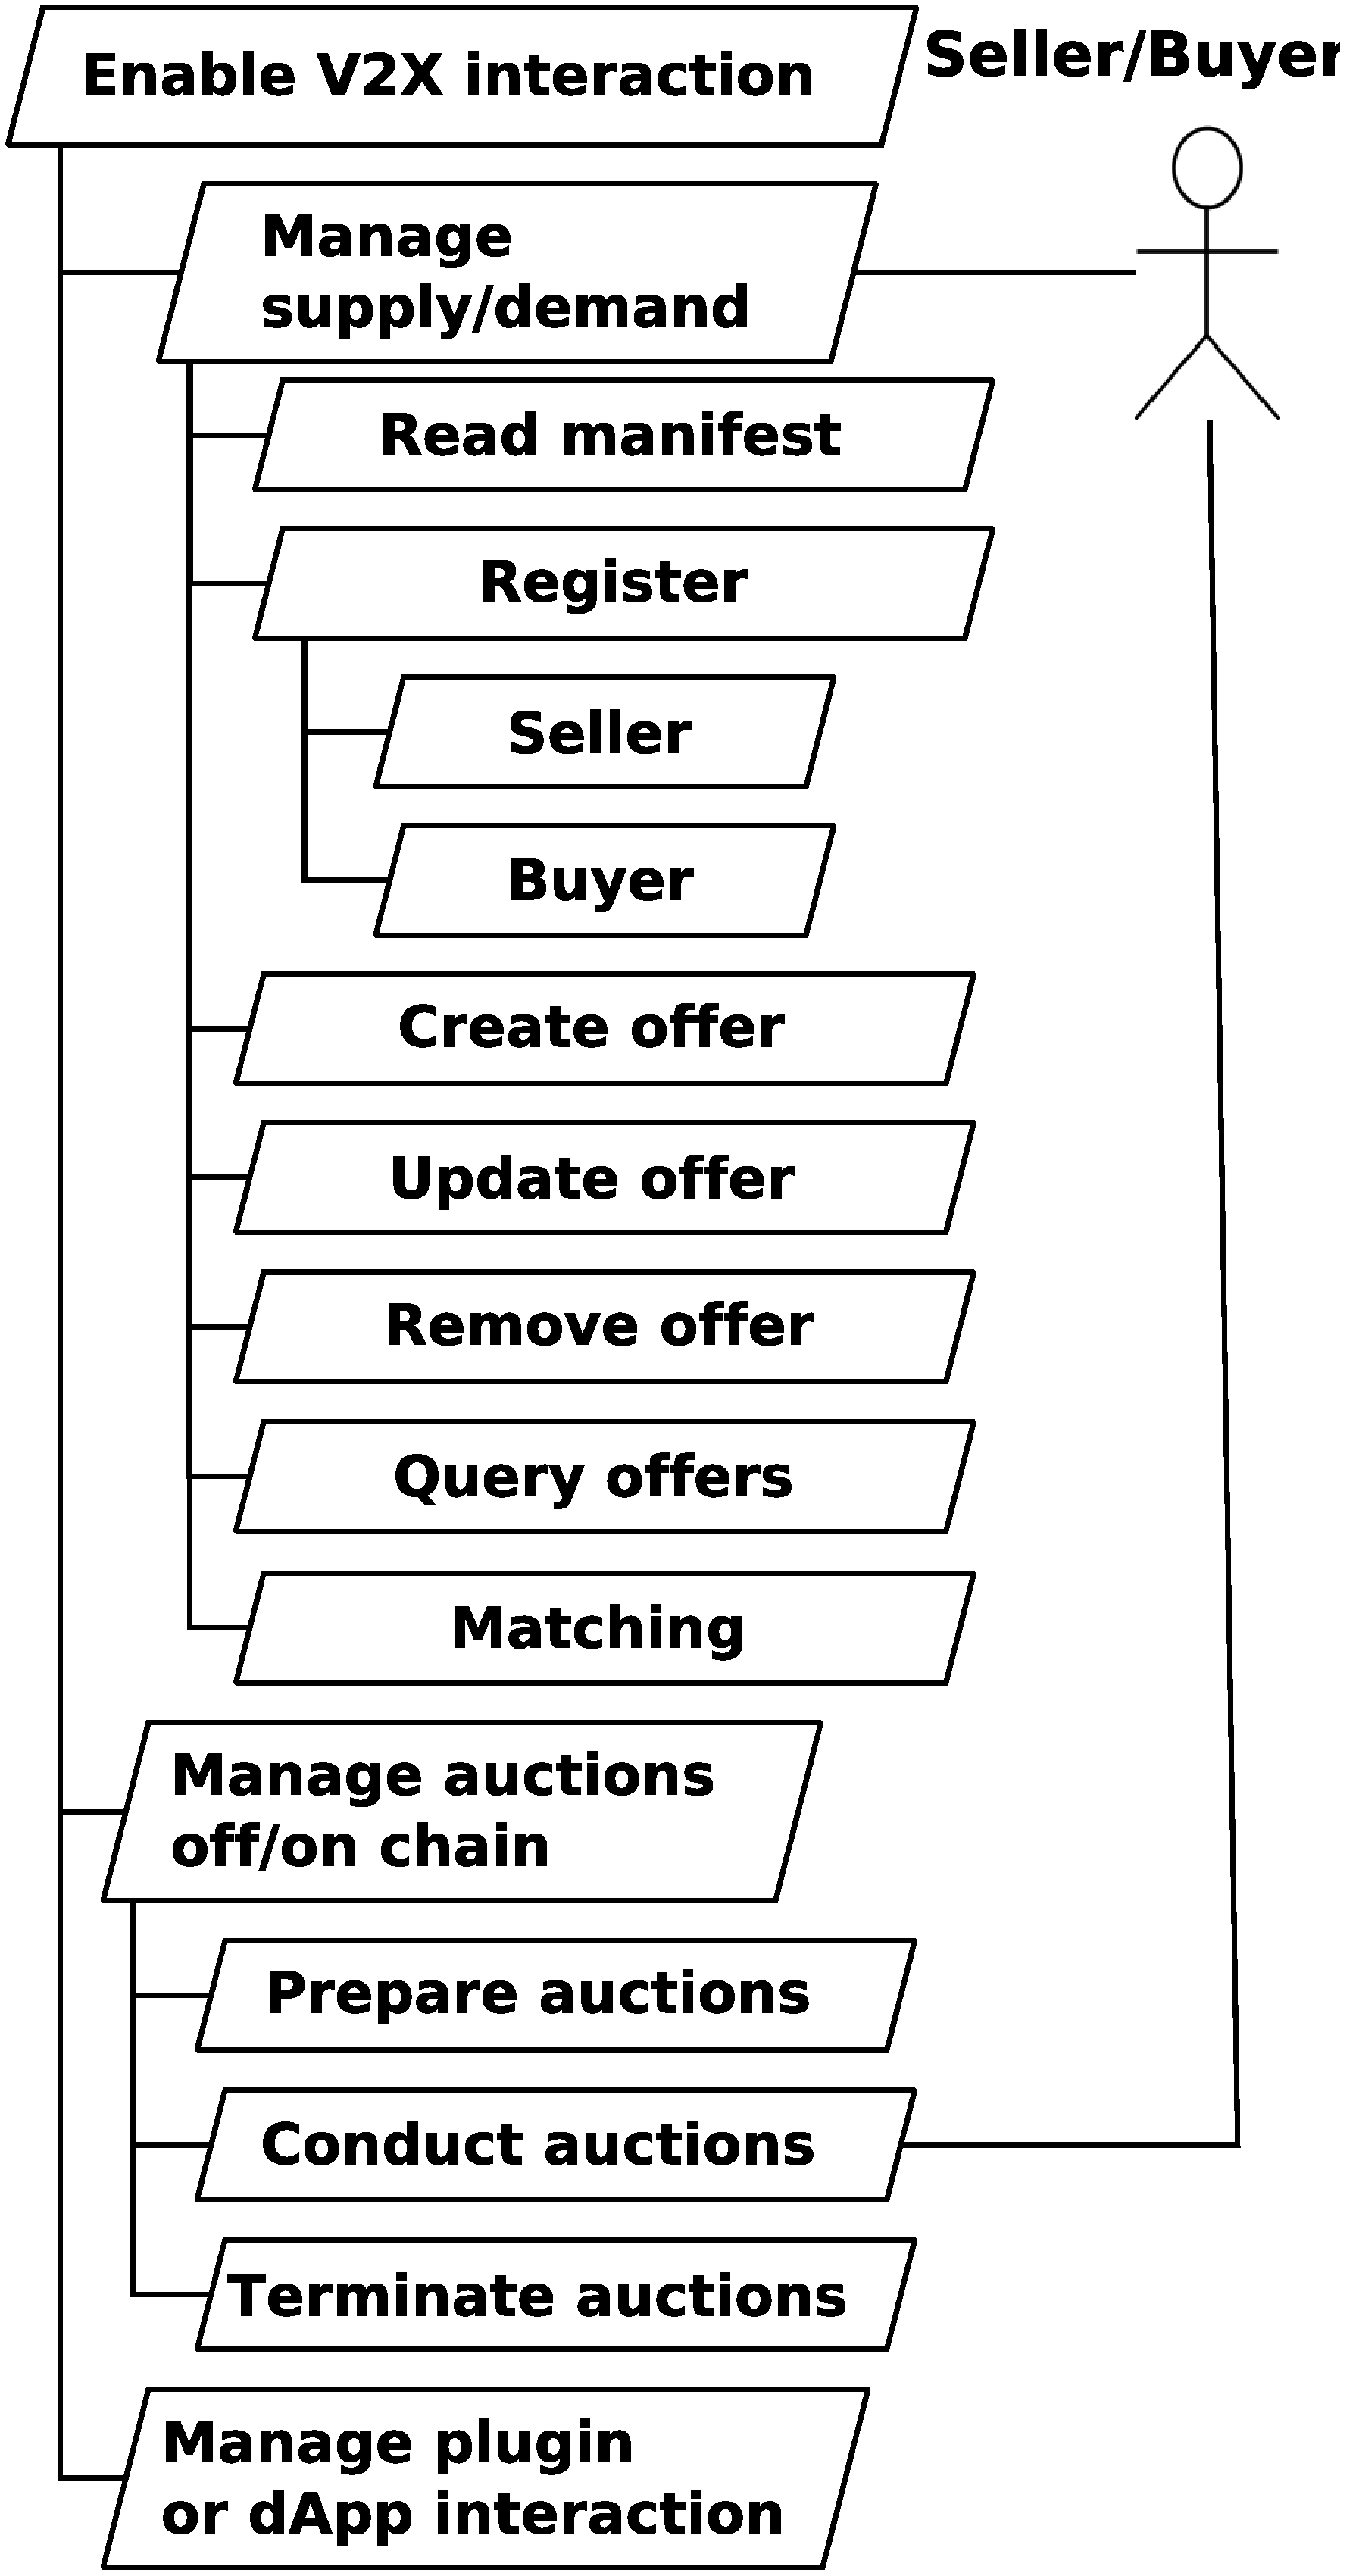
\includegraphics[scale=0.175]{Figures/aom/20180501_goal-model--refined-2.pdf}
%					\caption{Chorus - Goal model refinement \textit{Enable V2X interaction} (Source: Based on \cite{leidingM2M}).}	
%					\label{fig:refined-aom-goal-model-2}
%				\end{figure}				
%	
%				\begin{figure}[H]
%					\centering
%					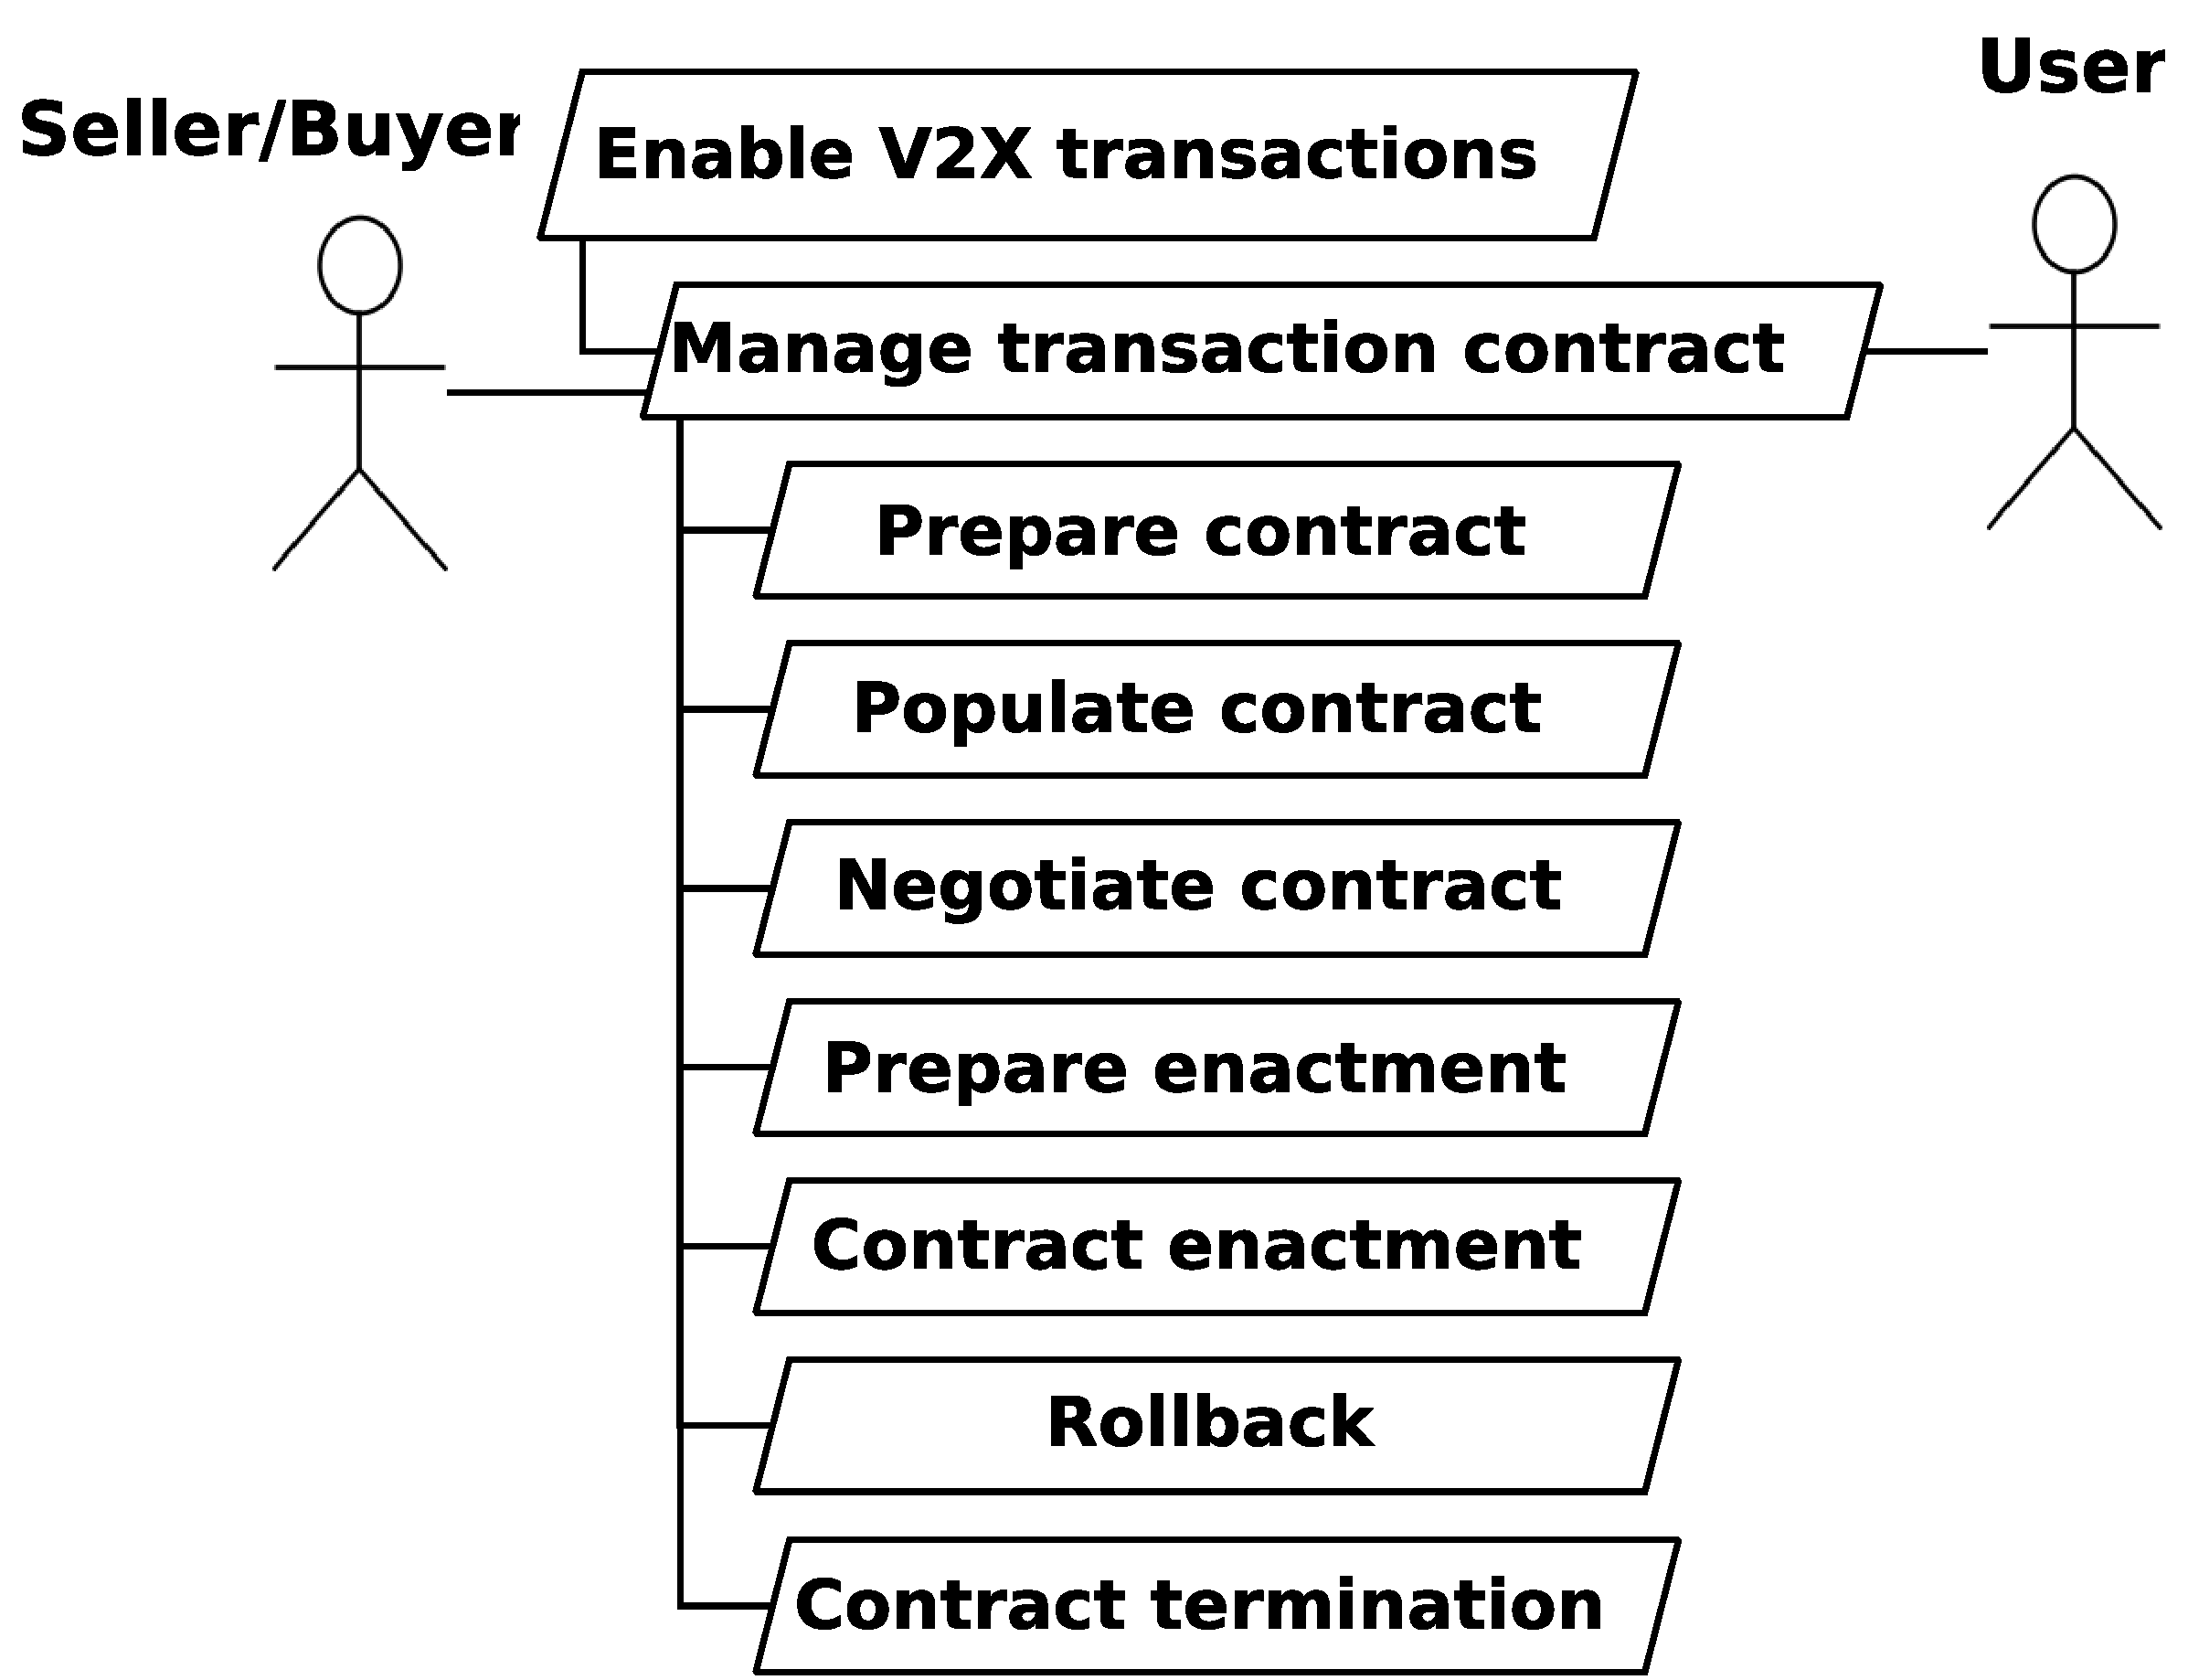
\includegraphics[scale=0.175]{Figures/aom/20180501_goal-model--refined-3.pdf}
%					\caption{Chorus - Goal model refinement \textit{Enable V2X transaction}  (Source: Based on \cite{leidingM2M}).}	
%					\label{fig:refined-aom-goal-model-3}
%				\end{figure}
%				
%				\begin{figure}[H]
%					\centering
%					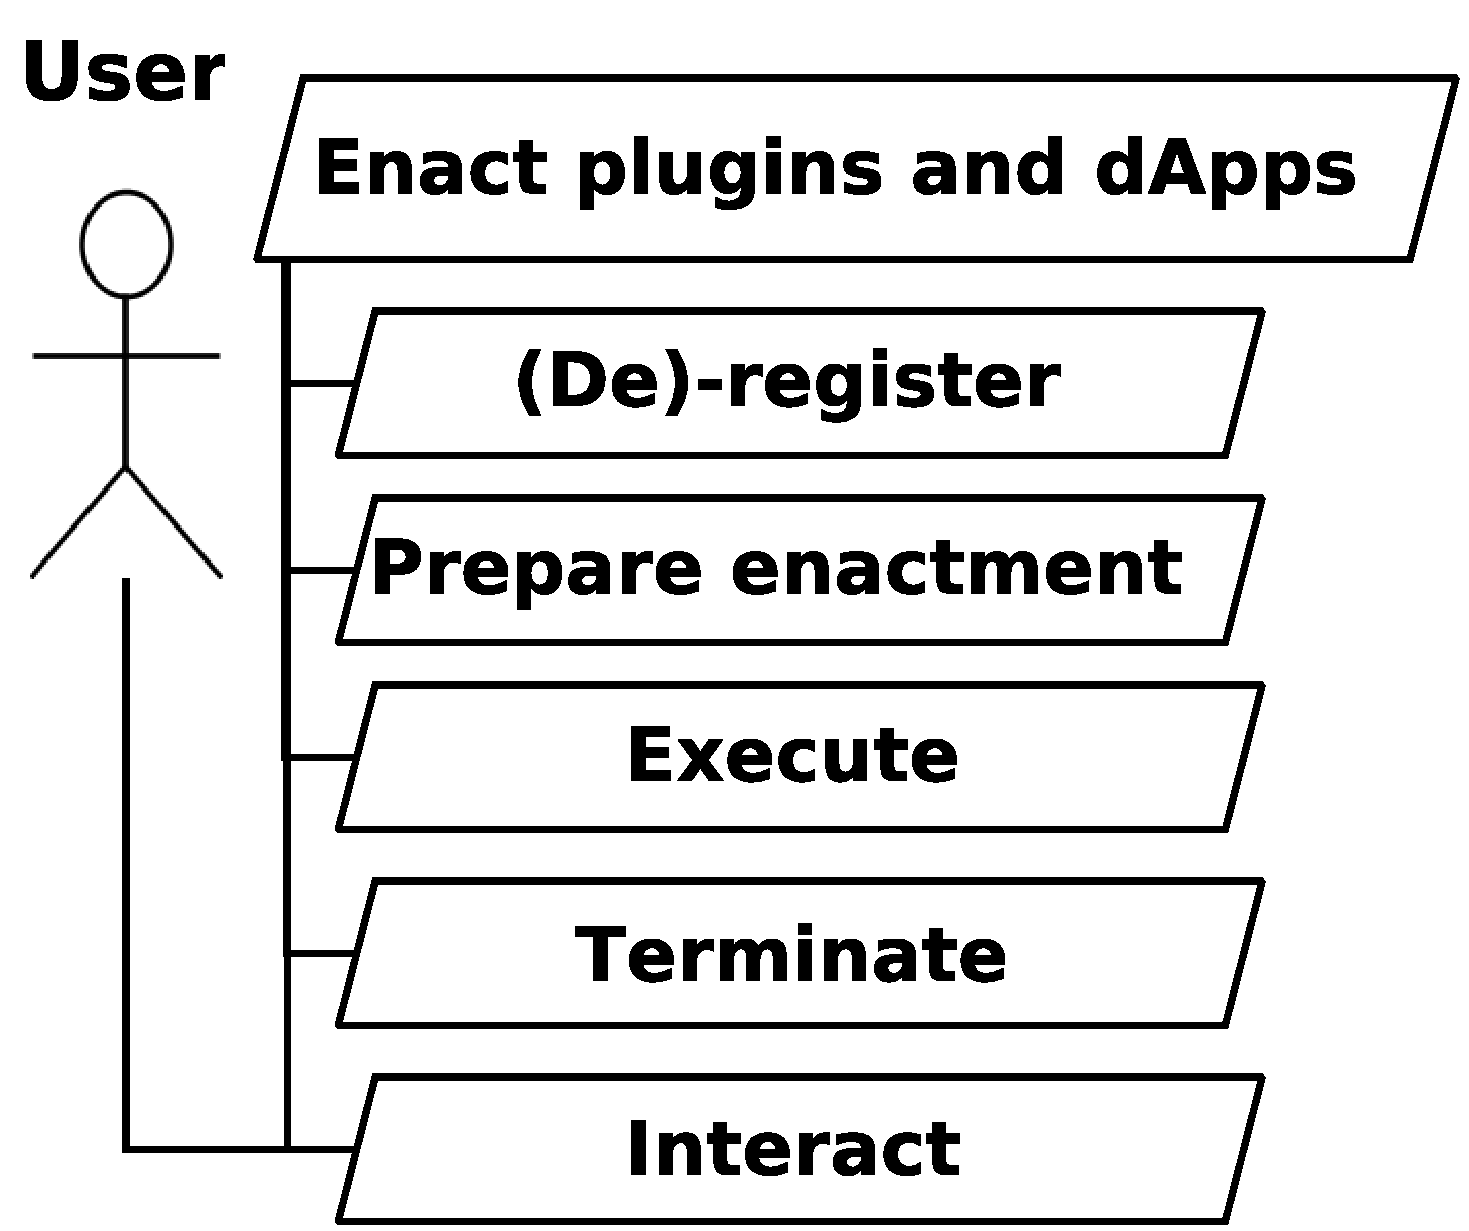
\includegraphics[scale=0.175]{Figures/aom/20180501_goal-model--refined-4.pdf}
%					\caption{Chorus - Goal model refinement \textit{Plugin and dApp enactment}.}	
%					\label{fig:refined-aom-goal-model-4}
%				\end{figure}


			The presented goal model is used in the following Section \ref{ss:component-diagrams} to derive our system architecture. We do not list all details of the further refined AOM goal model in this whitepaper due to space constraints and in order to focus on the most relevant system components and features.
									
			%% ----------------------------------------------------------------
			%% ----------------------------------------------------------------				

		%% ----------------------------------------------------------------
		%% ----------------------------------------------------------------	
		
		\subsection{Component Diagrams}
			\label{ss:component-diagrams}

			The abstract system- and business architecture is derived from the functional- and non-function requirements of the AOM goal model presented earlier. The services are powered by a service-oriented architecture (SOA) that is comprised of different designated components. Each of these components is self-contained, well-defined components and provides a specific set of services \cite{erl2005service}\cite{perrey2003service}. Dedicated services and components may also consist of other underlying sub-services \cite{rosen2012applied}. 
			
			In the following, a technology-agnostic UML-component-diagram representation is used to illustrate the system architecture \cite{booch1996unified}\cite{specification2007omg}. The UML notation elements used to model the architecture are presented in Figure \ref{fig:uml-component-diagram-overview}. In UML, components are represented as rectangular boxes and labeled either with the keyword \textit{component}, or with the component icon in the right-hand upper corner. A component may consists of further sub-components and is implemented by one, or more classes, or objects. Moreover, components are reusable and communicate via two types of interfaces as illustrated in Figure \ref{fig:uml-component-diagram-overview}. Small squares depict ports that are attached to the border of components and expose required and provided interfaces. Ports may also specify inputs and outputs as they operate uni-, or bi-directionally \cite{booch1996unified}\cite{specification2007omg}. Once more, sticky men are used to depict entities and their interactions with the system. 
			
			\begin{figure}[H]
				\centering
				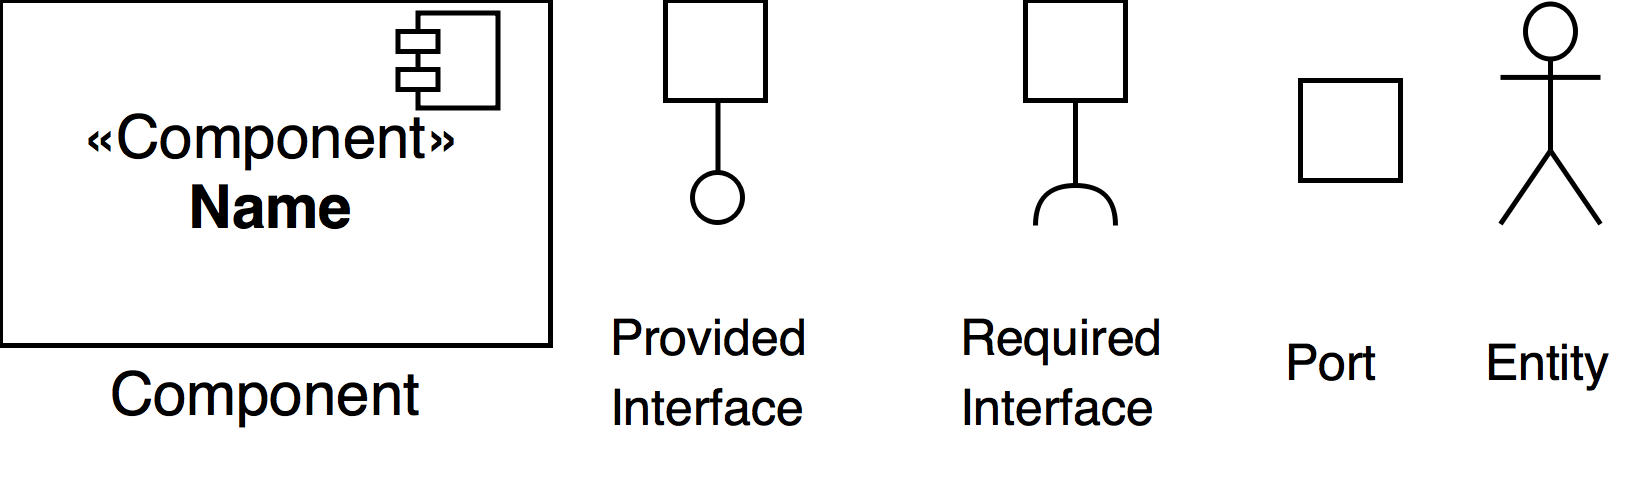
\includegraphics[scale=0.15]{Figures/UML-notation-elements.png}
				\caption{UML-component diagram notation elements.}	
				\label{fig:uml-component-diagram-overview}
			\end{figure}	
			
			The remainder of this section first introduces an abstract high-level overview of the system architecture and components. Afterwards, further illustration present selected sub-components of our architecture.
			
			\textbf{MAKE SURE TO ADAPT THE COMPONENT DIAGRAM TO THE AOM GOAL MODEL!}
			it is a distributed system that resides in differnt components on differnt places - hence we had to add further helper-component that enable communication and proper system execution.

			%% ----------------------------------------------------------------
			%% ----------------------------------------------------------------	

			\subsubsection{High-Level Architecture}
				\label{sss:high-level-architecture}

				\begin{figure}[H]
					\centering
					
\includegraphics[scale=0.4]{Figures/Dummy.jpg}
					\caption{Caption.}	
					\label{fig:high-level-architecture}
				\end{figure}				
			
			%% ----------------------------------------------------------------
			%% ----------------------------------------------------------------	
			

		%	\subsubsection{X}
		%		\label{sss:X}
			
			%% ----------------------------------------------------------------
			%% ----------------------------------------------------------------	


%	Notes
%		- foam
%		- a general technology section			
			


		%% ----------------------------------------------------------------
		%% ----------------------------------------------------------------	

		\subsection{Smart Contract Lifecycle Management}
			\label{ss:smart-contract-lifecycle-management}

			\textbf{Work-In-Progress}
			
			\begin{figure}[H]
				\centering
				
\includegraphics[scale=0.4]{Figures/Dummy.jpg}
				\caption{Caption.}	
				\label{fig:smart-contract-lifecycle-management}
			\end{figure}			
			
			%			The lifecycle of a micro lending contract is divided into the following stages: a) preparatory, b) negotiation, c) contract execution d) rollback and e) a contract expiry stage. During the preparatory stage, information about the involved entities, such as names and addresses are incorporated into the contract. In addition, the conditions of the requested loans are formally defined by specifying, e.g, the size of the loan, chosen currency, runtime and interest rates. The conditions of the requested loan mainly depend on information available to the lender, such as financial data gathered during previous interactions and transactions, personal data and information from social media. In case the borrower and the lender agree on the negotiated conditions, both parties sign the contract and express their approval - if no agreement is reached, a contract rollback is triggered. After signing the agreement, the contract execution phase is triggered and the lender transfers the loan to the borrower as illustrated in Figure \ref{fig:running-case-illustration}. Afterwards, the lender can use the loan to expand, or start a business. 
			%
			%			The micro lending contract terminates, or expires either after the defined loan timespan, or when the contract is prematurely terminated. The borrower pays back the loan either in separate rates, or as a whole, depending on the defined conditions. In addition, the lender also receives a fee, or an interest rate from the borrower for providing the loan. In case the borrower fulfills all his/her duties, the lender might provide a larger loan in the future based on the positive credit history of the borrower. Everex does not operate on the basis of P2P loans and instead invests its own aggregated capital to provide globally accessible credit services. Nevertheless, it is up to each Cryptocash owner to lend his/her own tokens to other users.	

		%% ----------------------------------------------------------------
		%% ----------------------------------------------------------------	
		
		\subsection{Library / API}
			\label{ss:library-api}				

			\textbf{Work-In-Progress}
			
		%% ----------------------------------------------------------------
		%% ----------------------------------------------------------------	

	%% ----------------------------------------------------------------
	%% ----------------------------------------------------------------
	
	\section{System Engagement Processes}
		\label{s:section-5}	
	
		%% RQ-3: What are the system-engagement processes for the stakeholders?
	
		Intro
		
		%describe processes here similar to evx paper

		%% ----------------------------------------------------------------
		%% ----------------------------------------------------------------	

		\subsection{Sequence Diagrams | or BPMN representation of Processes}

			\textbf{Work-In-Progress}

			\begin{figure}[H]
				\centering
				
\includegraphics[scale=0.4]{Figures/Dummy.jpg}
				\caption{Caption.}	
				\label{fig:sequence-diagram-1}
			\end{figure}


		%% ----------------------------------------------------------------
		%% ----------------------------------------------------------------	
		
		\subsection{Auction Algorithm}
			\label{ss:auchtion-algorithm}				

			\textbf{Work-In-Progress}
			
			Vickrey auction \cite{ausubel2006lovely}\cite{lucking2000vickrey}
			
			Auction stuff that might happen during road-space negotiations as described in Section~\ref{ss:V2V}

			1-1 auction
			Note:
			-Vickrey Auction
			- Buyer max price: 3€
			Seller min price: 2.80€
			- only one auction round
			- Note: If seller offer > buyer offer => no deal
			
			\begin{figure}[H]
				\centering
				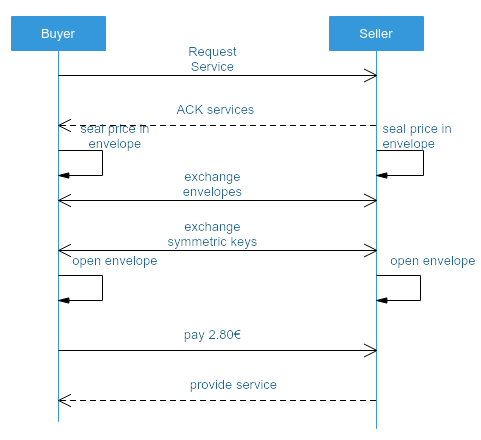
\includegraphics[scale=0.4]{Figures/auction/20180501_auction-aglorithms--1-to-1.png}
				\caption{Caption.}	
				\label{fig:auction-algorithm-1-1}
			\end{figure}
			
			X-X auction
			Note: 
			- (modified) Vickrey Auction
			- only one auction round
			- buyer-1 max price:1.80
			- buyer-2 max price: 3.20
			- buyer-3 max price: 3.5
			- seller min price: 2.0
			- Note: If seller offer > buyer offer => no deal
			- NOTE: In case we have multiple sellers, the workflow is similar. In the end, the highest bidder is matched with the seller of the highest price, the second highest offer with the second highes seller price ... and so on. Please keep in mind that this is a vickrey auction => hence, highest bidder pay price of the second highest offer and so on...

			\begin{figure}[H]
				\centering
				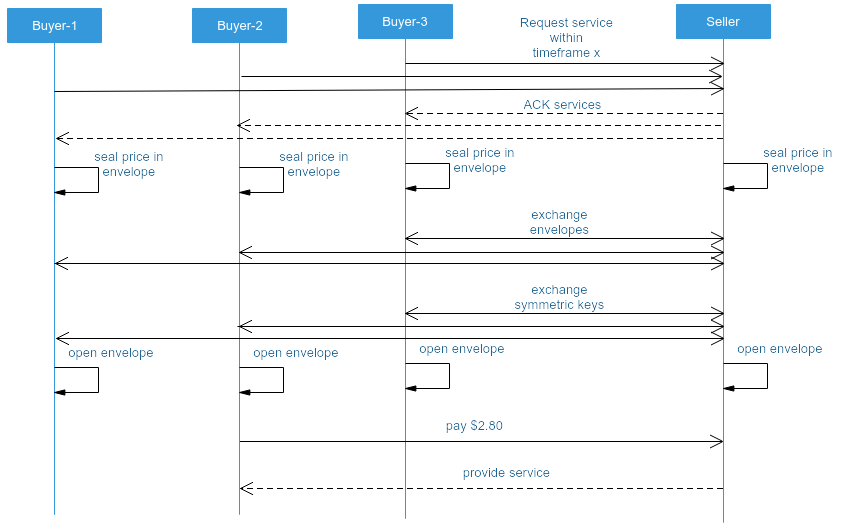
\includegraphics[scale=0.4]{Figures/auction/20180501_auction-aglorithms--X-to-X.png}
				\caption{Caption.}	
				\label{fig:auction-algorithm-X-X}
			\end{figure}			

		%% ----------------------------------------------------------------
		%% ----------------------------------------------------------------	

		\subsection{Token Economics and Value Proposition}

			\textbf{Work-In-Progress}
					
		%% ----------------------------------------------------------------
		%% ----------------------------------------------------------------	

	%% ----------------------------------------------------------------
	%% ----------------------------------------------------------------

	\section{Prototype and Feasibility Study}
		\label{s:section-6}	
			
		Intro
		
		%% ----------------------------------------------------------------
		%% ----------------------------------------------------------------	
		
		\subsection{Prototype}
			\label{ss:protoype}				

			\textbf{Work-In-Progress}
			
					
		%% ----------------------------------------------------------------
		%% ----------------------------------------------------------------	
		
		\subsection{Evaluation}
			\label{ss:evaluation}				

			\textbf{Work-In-Progress}
			
					
		%% ----------------------------------------------------------------
		%% ----------------------------------------------------------------			

	%% ----------------------------------------------------------------
	%% ----------------------------------------------------------------

	\section{Discussion}
		\label{s:section-7}	
		
		Intro

		%% ----------------------------------------------------------------
		%% ----------------------------------------------------------------	
		
		\subsection{Critical Analysis}
			\label{ss:critical-analysis}
							
			\textbf{Work-In-Progress}		
		
		%% ----------------------------------------------------------------
		%% ----------------------------------------------------------------			
		
		\subsection{Related Work}
			\label{ss:competitor-analysis}
			
			%Competitor analysis (will)				

			\textbf{Work-In-Progress}

%			Several other academic as well as non-academic projects experimented with ideas and prototypes of blockchain-based trading platforms that enable the M2M economy. In \cite{leiding2016self}, the authors describe a blockchain solution for a variety of services within vehicular ad-hoc networks (VANETs), e.g., traffic management, toll payment systems, traffic regulation enforcement and more. In 2018, the automotive company got a patent for a very similar idea of traffic marshaling via a blockchain system \cite{macneille2018vehicle}. Chorus technologies \cite{chorusWhitepaper} envisioned a whole library for all types of services and transaction around the ecosystem of autonomous vehicles within VANETs. The authors of \cite{davWhitepaper} propose a solution that allows vehicles to discover, communicate and transact with one another using cryptocurrencies. 
%			\cite{oakenTeslaTollbooth} present a prototype of a blockchain-based toll road system. In 2013, Mike Hearn gave a short talk\footnote{\url{https://www.youtube.com/watch?v=MVyv4t0OKe4}} at the Turing Festival in Edinburgh describing several of these ideas. 
%			
%			Besides the automotive sector, the authors of \cite{sikorski2017blockchain} describe and implement a M2M electricity market for chemical industry where industrial plants are trading electricity with each other via a blockchain platform.
%			
%			The alternative blockchain solution IOTA is offering an IoT market place \cite{iotaMarketplace} for IoT devices where sensor data can be bought and sold using blockchain technology.
%			
%		

%%DAV MVPs \cite{davWhitepaper}
%%MVP#1 World’s first autonomous vehicle to autonomously bid for delivery services, complete them, and get paid using tokens directly to its own wallet.
%%MVP #2 World’s first autonomous vehicle to pay for its own battery replacement using tokens and take off to complete its delivery mission.
%%
%%MVP #3 World’s first autonomous vehicle to pay another autonomous vehicle (robot) using tokens for completing the last mile of a delivery mission.
%%
%%MVP #4 Longest drone delivery flight ever, flying cross-country using the support of multiple DAV battery-changing stations along the way.

% we also have talk about XAIN

% https://slock.it/


%			
%Direct Competitors: 
%
%1. https://www.oakeninnovations.com/
%Straights: first on the market, working SW and HW prototypes, solid development and r&d team, lead developer joined Ethereum, support from car manufacturers, won multiple startup competitions. 
%
%Weaknesses: dependent on in-car hardware nodes, architecture lacks scalability. 
%
%2. https://swarm.city/
%Straights: early in the ethereum community, major ethereum contributors, lots of connections, conducted successful ICO
%
%Weaknesses: Absolutely not scalable due to all logic being put on Ethereum Blockchain, no scalability solution, lost all the funds from ICO in the Parity Hack (one of a few projects who didn't get their money back), bad history with their early CEO (formerly Arcade City), radical anarchists.
%
%3. http://www.flyingcarpet.network/
%Straights: early working prototype, presented his project at Devcon 3
%
%Weaknesses: Focused on Drones.
%
%4. https://dav.network/
%Straights: A lot of marketing materials and ICO coverage, financial resources, large dev team, many connections in Ethereum community including Bancor and Dr. Greg Colvin – EVM core dev., working prototypes. 
%
%Weaknesses:
%Very vague idea with no modern use, not able to generate any value or revenue. 			
		
		%% ----------------------------------------------------------------
		%% ----------------------------------------------------------------					
	
	%% ----------------------------------------------------------------
	%% ----------------------------------------------------------------

	\section{Conclusion and Future Work}
		\label{s:section-8}	

		We conclude ...
		
		\textbf{Work-In-Progress}		
		
		
		%Future Work
		%	- mention the academic M2M paper?
		%	- chorus long term vision
				
	%% ----------------------------------------------------------------
	%% ----------------------------------------------------------------


	\label{Bibliography}
	\bibliographystyle{splncs03}
	\bibliography{Bibliography}
	
	%% ----------------------------------------------------------------
	%% ----------------------------------------------------------------	



	%
\end{document}


%%%%%%%%%%%%%%%%%%%%%%%%%%%%%%%%%%%%%%%%%%%%%%%
%
%	Notes
%		- foam
%		- a general technology section
%
%
%
%
%
%
%
%
%


